Schéma objet-relationnel / 100\% relationnel.

Discussion sur pourquoi 100\% relationnel ?! ORM ?! Doctrine / Symfony ?

Présentation des templates / formulaires

\section{Schémas relationnelles}
\subsection{Schéma objet-relationnel}
\subsection{Schéma relationnel pur}
\begin{description}
\item[TERME](\underline{lib\_terme})
\item[CONCEPT](\underline{terme\_vedette}\up{\#}, concept\_general\up{\#})
\item[SYNONYME](\underline{terme\up{\#}, concept\up{\#}})
\item[ASSOCIATION](\underline{concept1\up{\#}, concept2\up{\#}})
\end{description}
\subsection{Discussion}

\section{Pourquoi un ORM ?}

\section{Décisions}
\subsection{Templates et formulaires}

\subsubsection{Accueil}
\begin{figure}[H]
\begin{center}
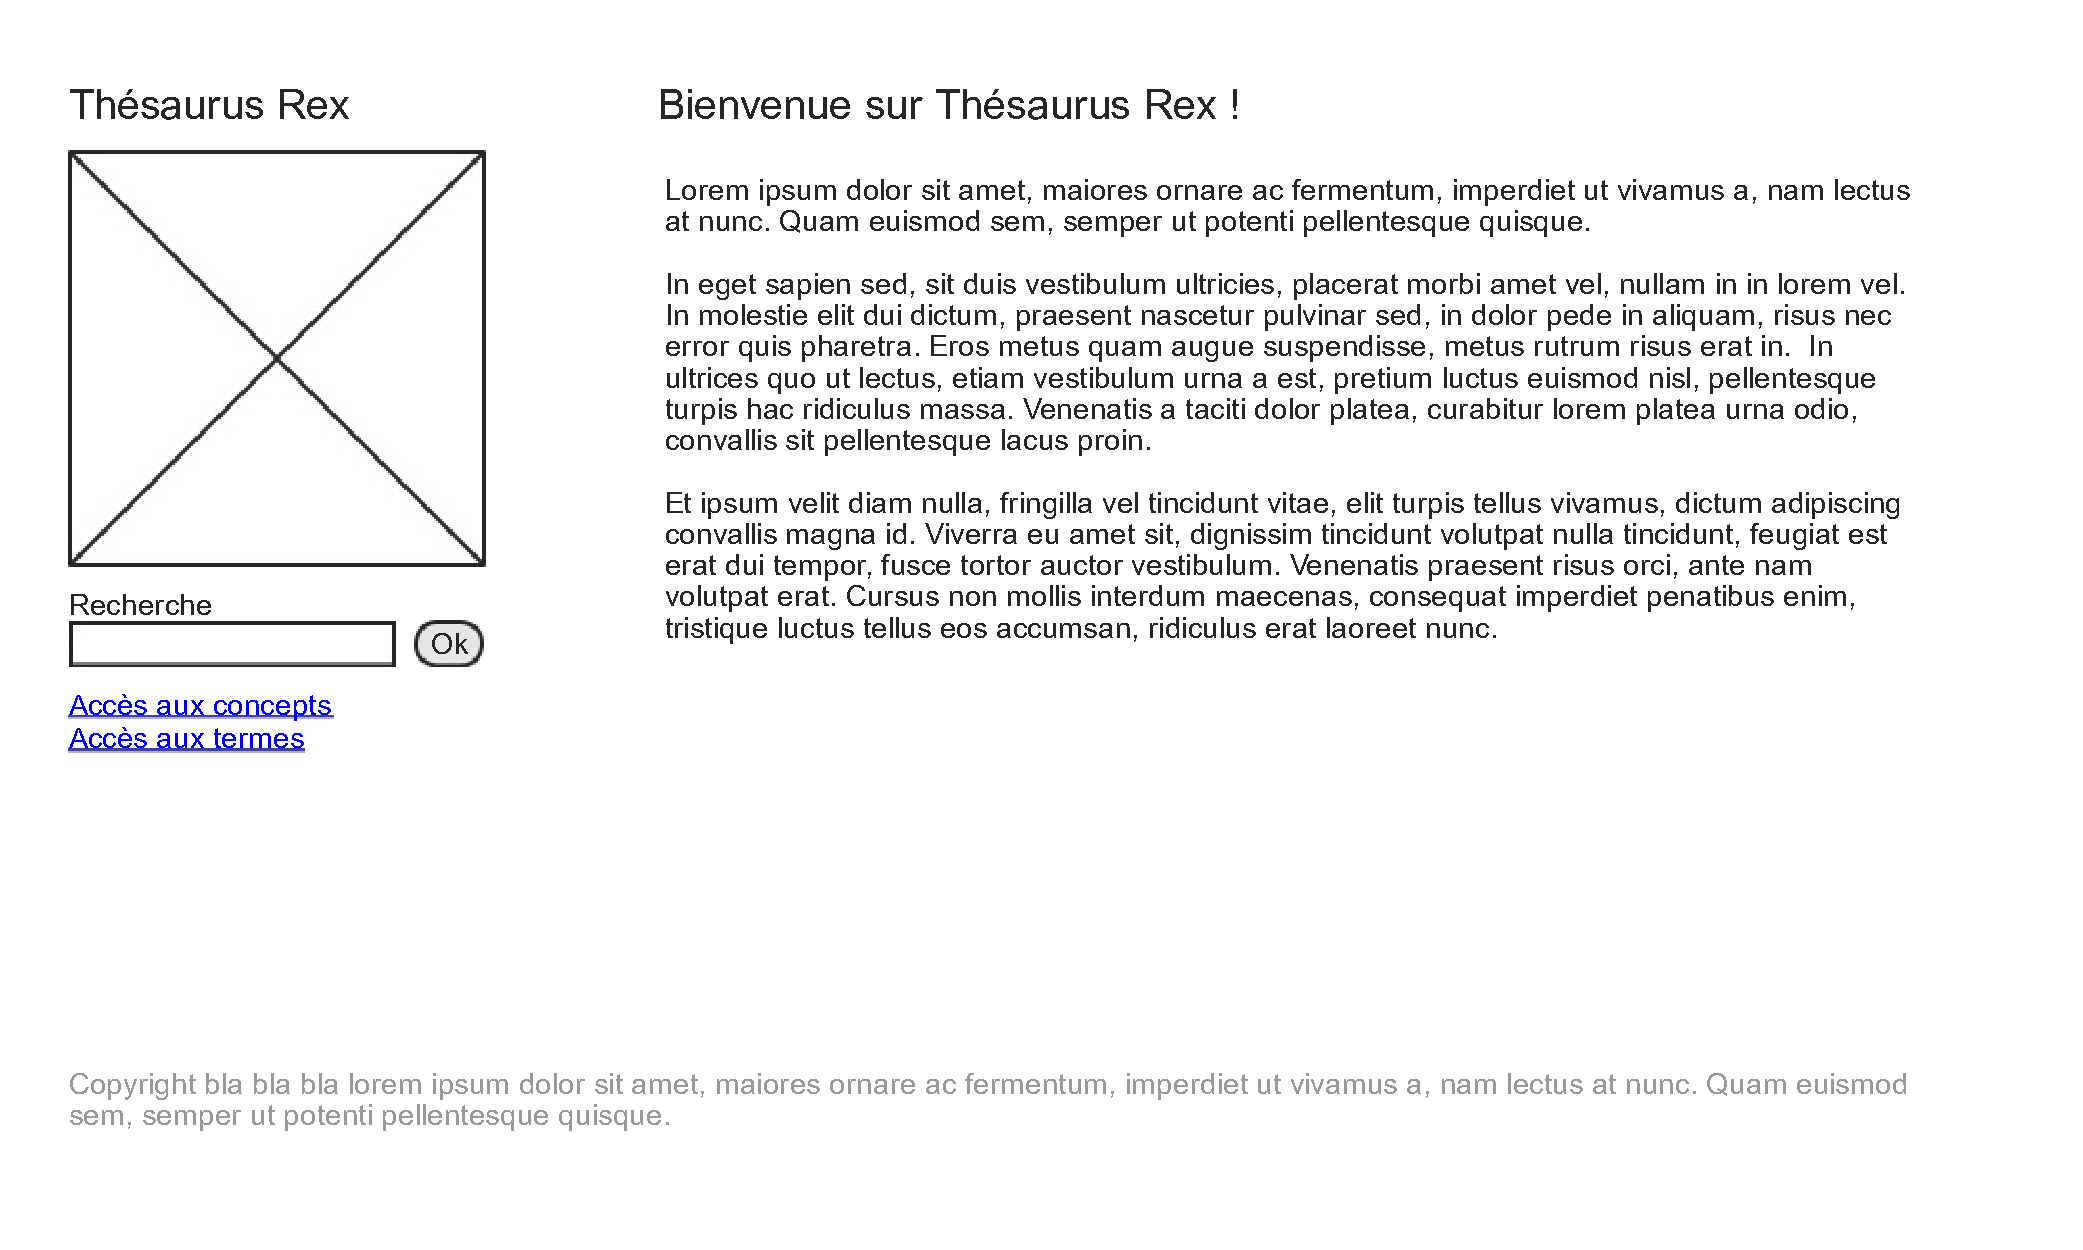
\includegraphics[width=\textwidth]{files/template_accueil}
\end{center}
\caption{Template de la page d'accueil de Thésaurus Rex.}
\end{figure}

\subsubsection{Vue hiérarchique des concepts}
\begin{figure}[H]
\begin{center}
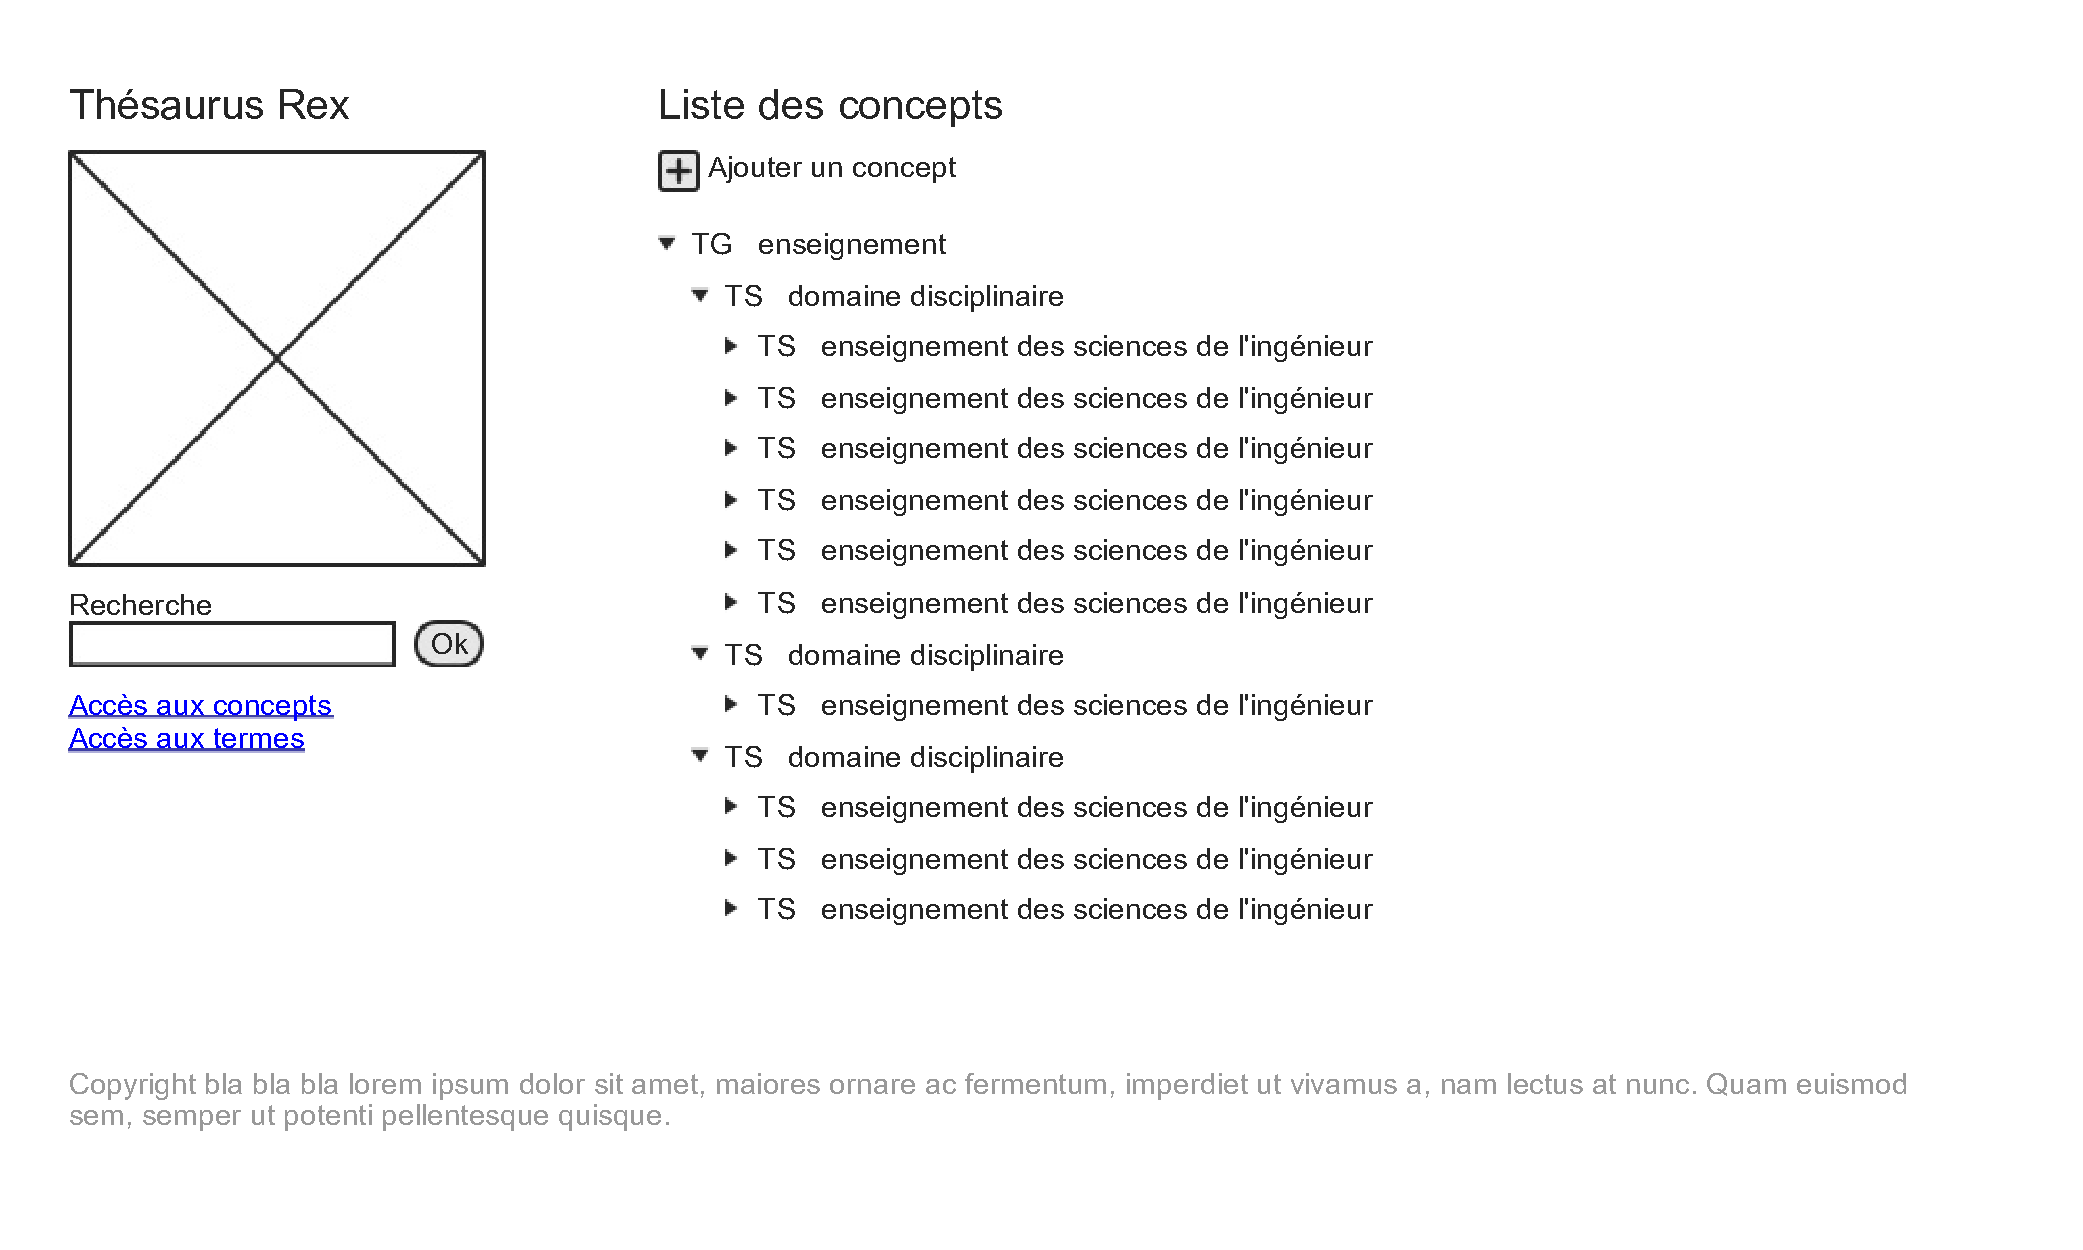
\includegraphics[width=\textwidth]{files/template_concepts}
\end{center}
\caption{Template de la vue hiérarchique des concepts.}
\end{figure}

\subsubsection{Visualisation d'un concept}
\begin{figure}[H]
\begin{center}
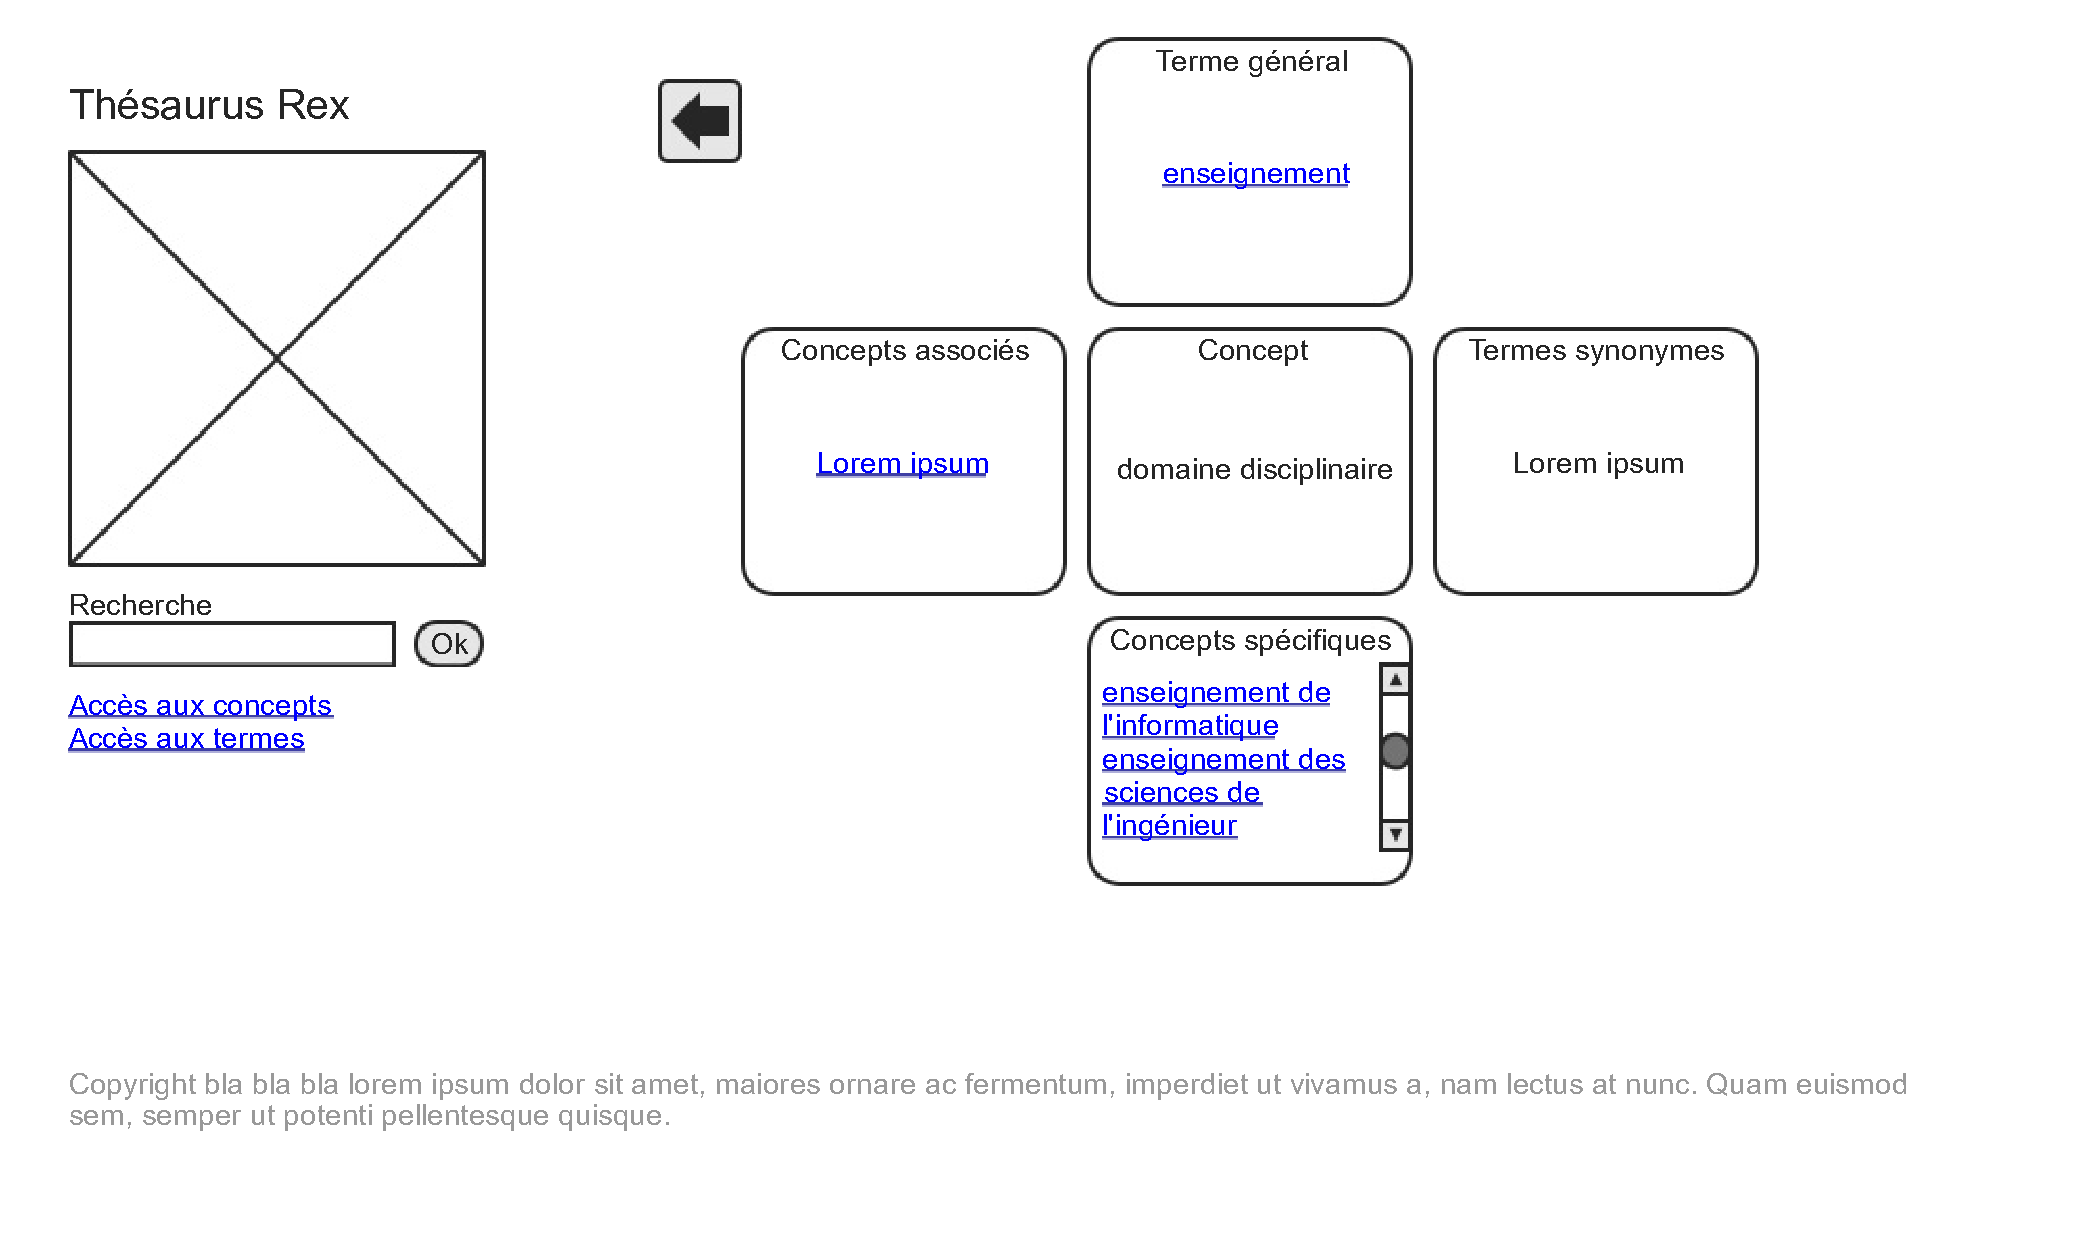
\includegraphics[width=\textwidth]{files/template_concept}
\end{center}
\caption{Template d'affichage d'un concept.}
\end{figure}

\subsubsection{Ajout / Édition d'un concept}
\begin{figure}[H]
\begin{center}
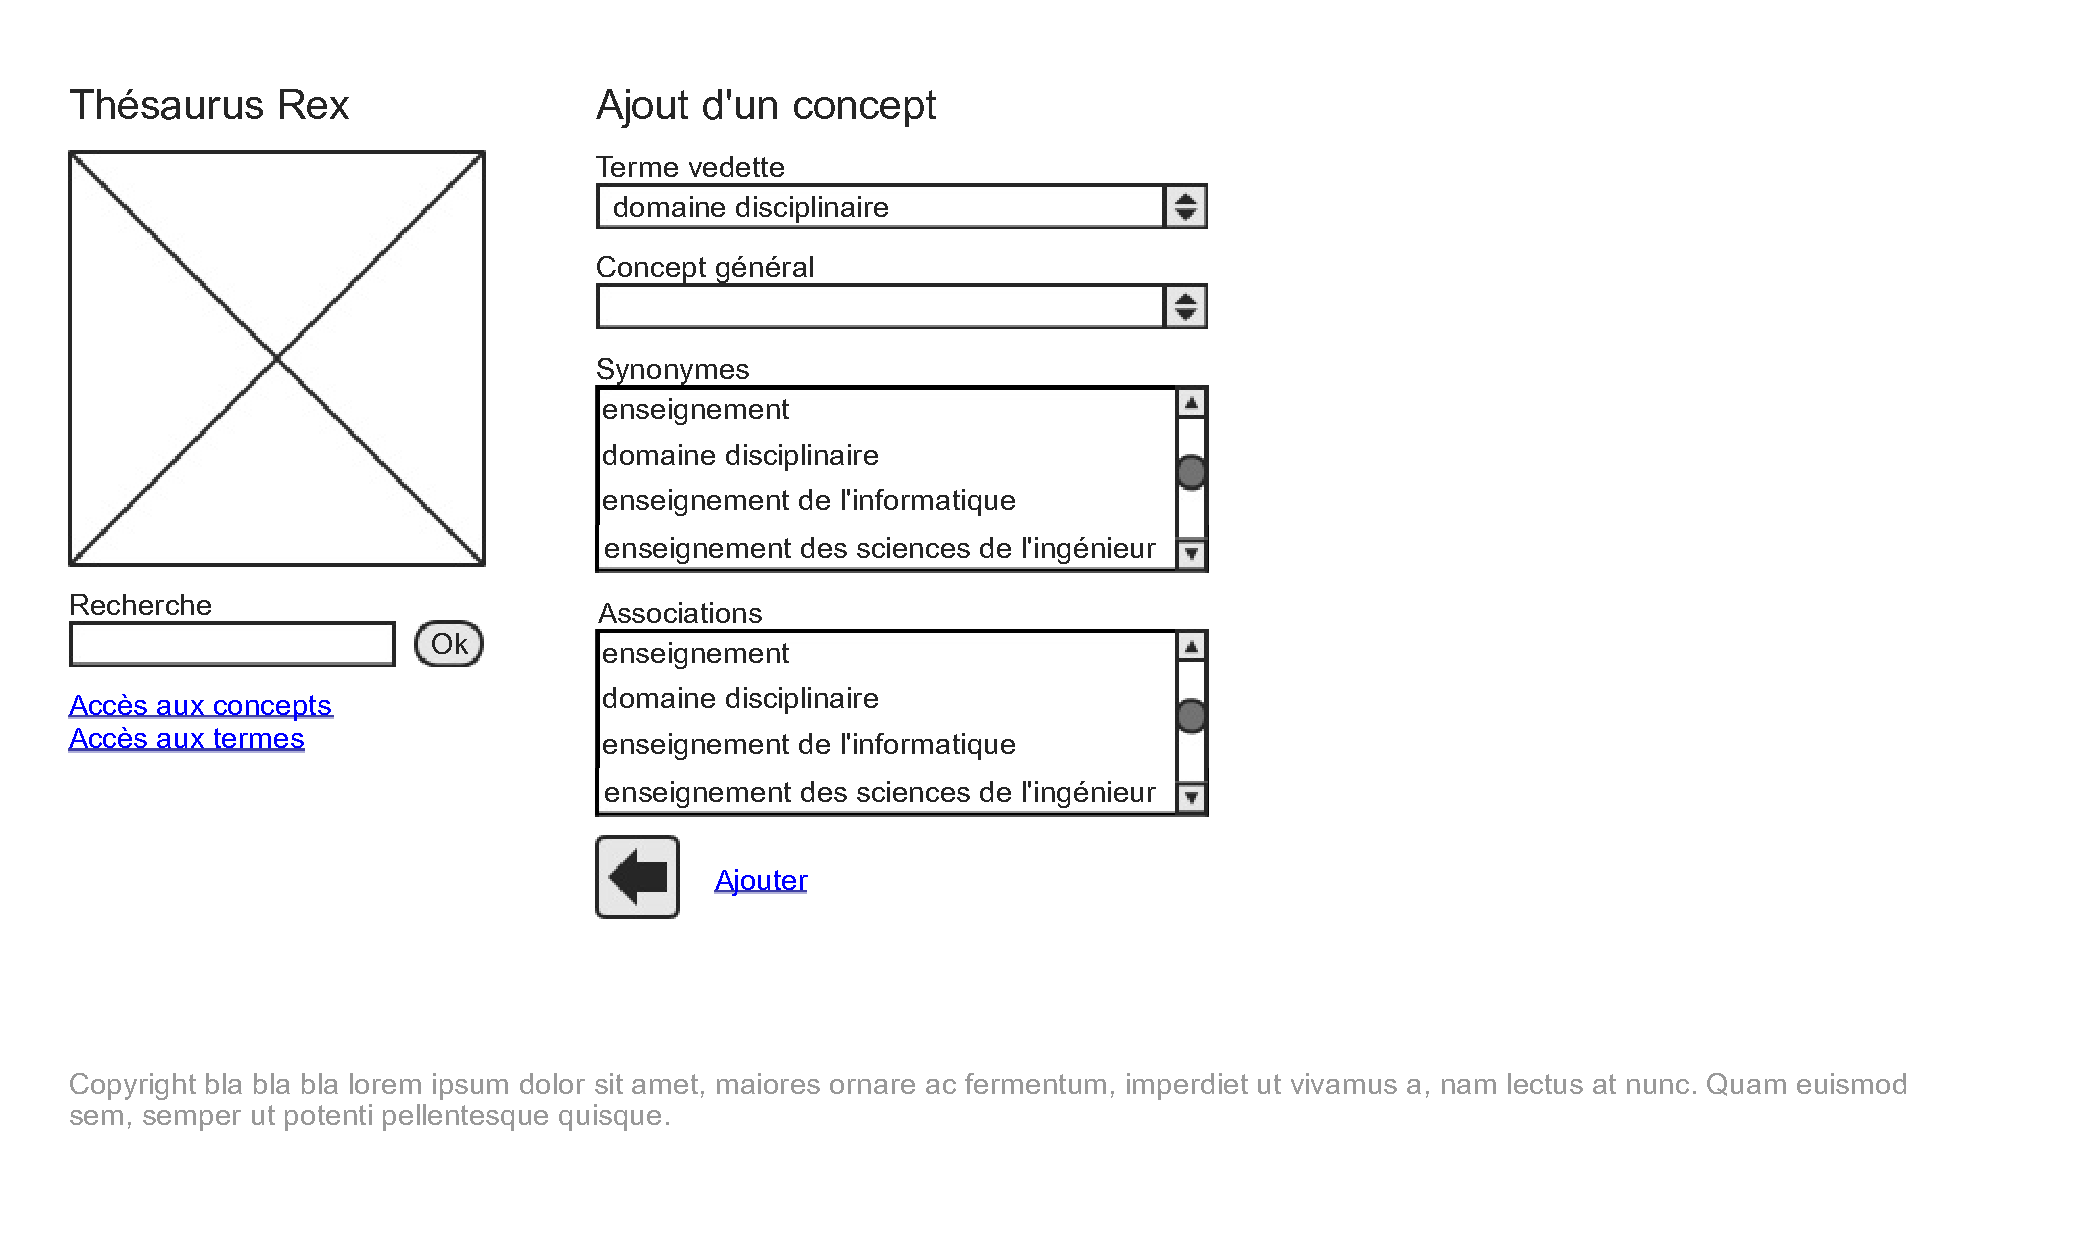
\includegraphics[width=\textwidth]{files/template_concept_add}
\end{center}
\caption{Template du formulaire d'ajout d'un concept.}
\end{figure}
\begin{figure}[H]
\begin{center}
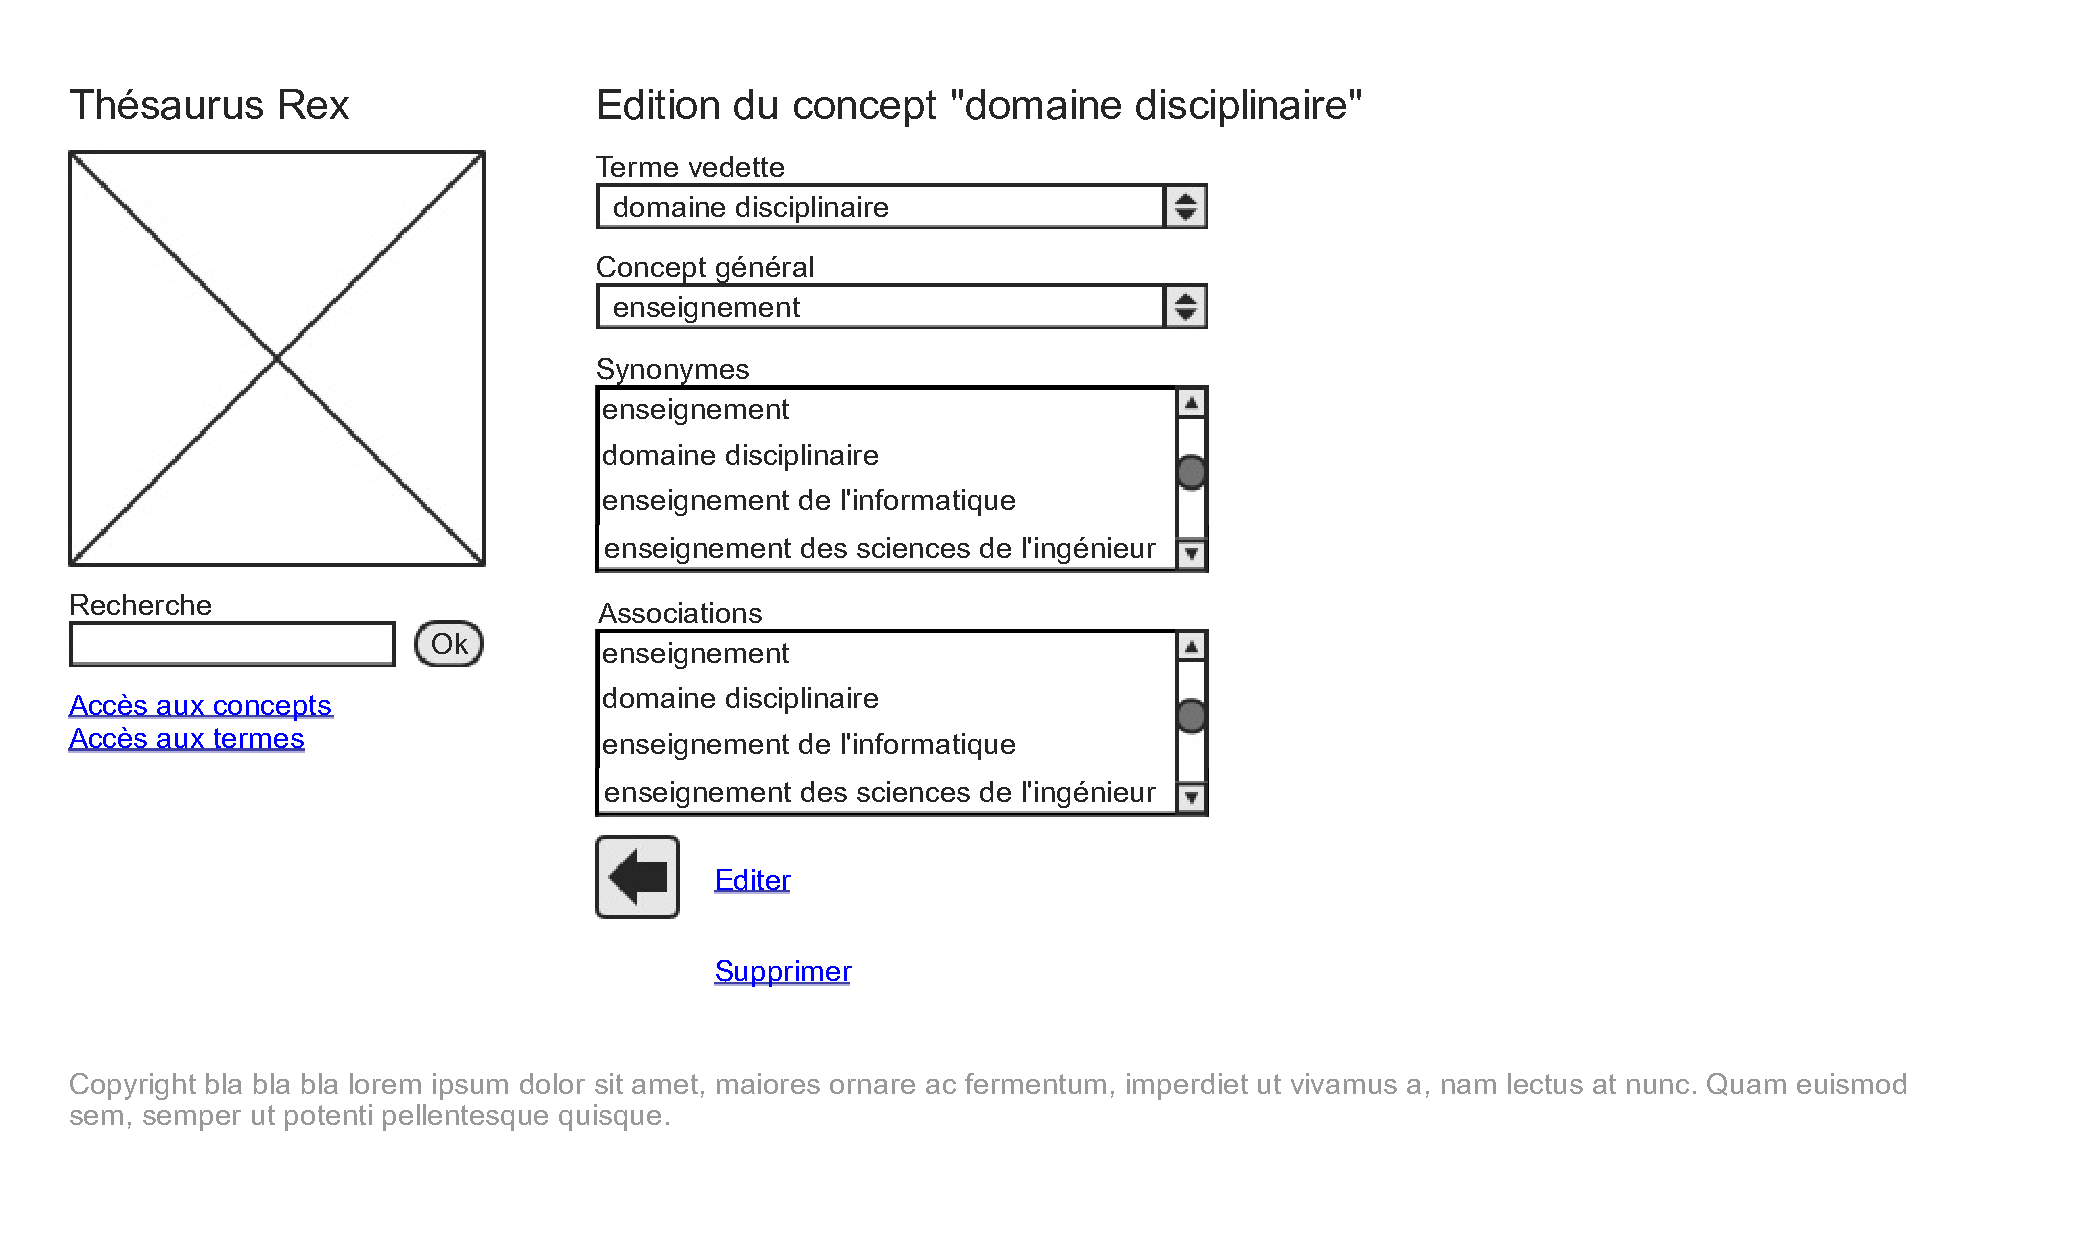
\includegraphics[width=\textwidth]{files/template_concept_edit}
\end{center}
\caption{Template du formulaire d’édition d'un concept.}
\end{figure}

\subsubsection{Liste des termes}
\begin{figure}[H]
\begin{center}
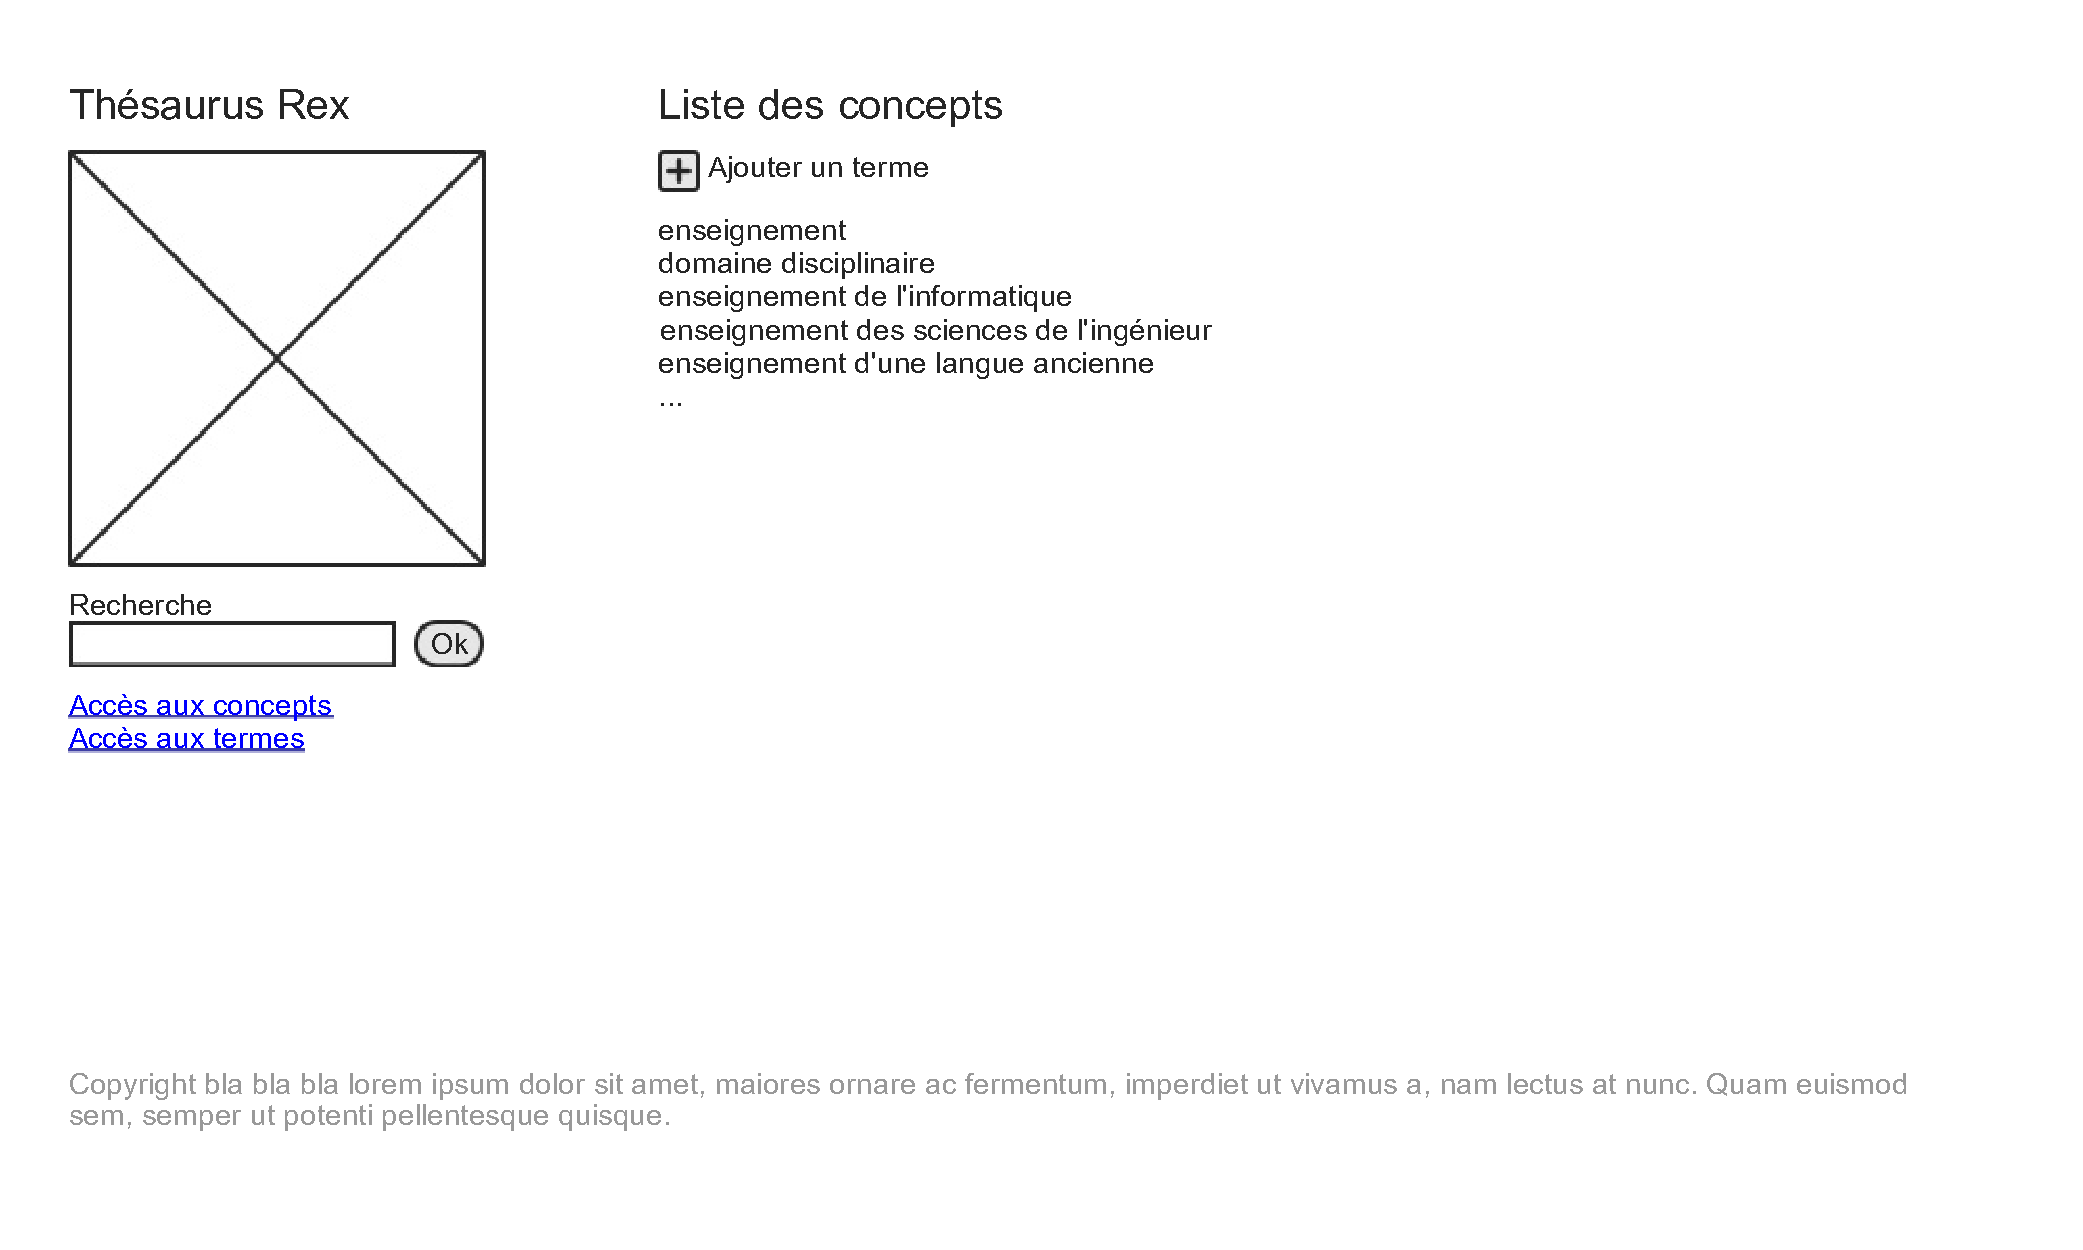
\includegraphics[width=\textwidth]{files/template_termes}
\end{center}
\caption{Template de visualisation des termes.}
\end{figure}

\subsubsection{Édition d'un terme}
\begin{figure}[H]
\begin{center}
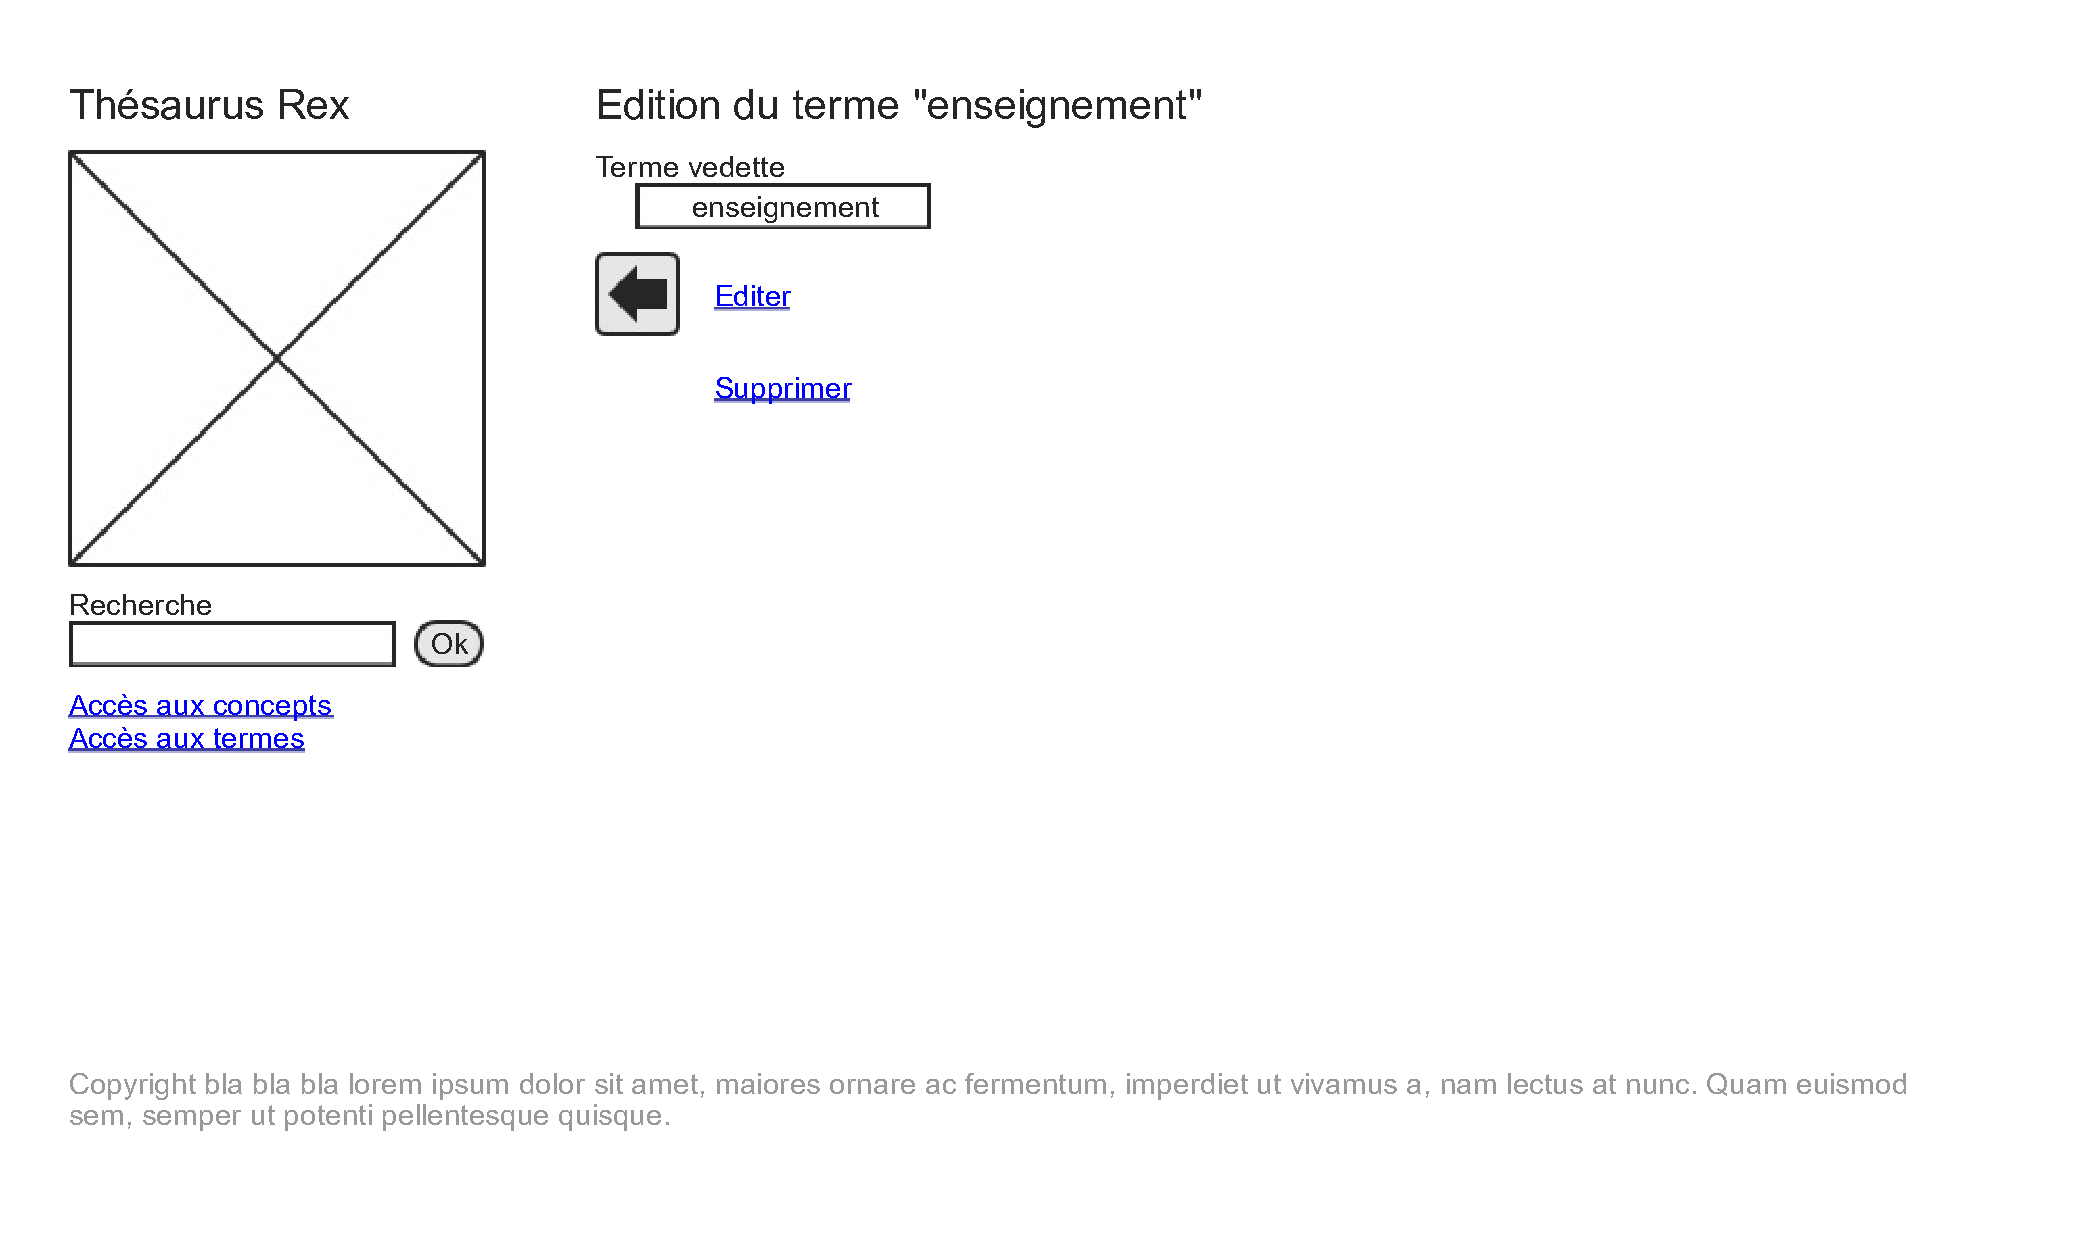
\includegraphics[width=\textwidth]{files/template_terme_edit}
\end{center}
\caption{Template du formulaire d'ajout d'un concept.}
\end{figure}


\subsection{Framework}